\documentclass[12pt, oneside]{extbook}

\usepackage{geometry}
\usepackage{graphicx}
\usepackage{listings}
\usepackage[dvipsnames]{xcolor}
\usepackage[italian]{babel}
\usepackage{amssymb}
\usepackage{mathrsfs}
\usepackage{amsmath}

\geometry{
	a4paper, 
	top = 2cm,
	left = 1.5cm,
	right = 1.5cm,
	bottom=2cm
}
\lstset{
	language=Python, 
	%frame=shadowbox,
	%rulesepcolor=\color{gray!50},
	basicstyle=\ttfamily\small,
	keywordstyle=\color{purple}\bfseries\small,
	stringstyle=\color{ForestGreen}\small,
	commentstyle=\color{blue}\small,
	numbers=left,
	numberstyle=\small\color{black},
	numbersep=5pt,
	tabsize=2,
	showtabs=false,
	showspaces=false,
	showstringspaces=false,
	%escapechar=|,
	%captionpos=b,
	breaklines=true,
	keepspaces=true
}

\title{Machine Learning}
\author{Pierciro Caliandro}

\begin{document}
\maketitle
\tableofcontents
\chapter{Introduzione del corso}
\section{Introduzione}
Per il progetto: sviluppare	un notebook in cui la parte espositiva sia presente, quindi intercalare markdown + codice, dove il markdown deve esserci e deve essere eloquente.\\NON solo codice, esporre i ragionamenti, le limitazioni etc...\\
\section{Presentazione del ML}
L'informatica è risolvere problemi da un punto di vista algoritmico, risolvere un problema attraverso algoritmi si può dividere in fasi:
\begin{itemize}
	\item analizzare il problema
	\item vederlo in modo matematico
	\item pensare ad un algoritmo
	\item implementarlo in un linguaggio
	\item verificare la correttezza (attività di testing) e valutarne l'efficienza
\end{itemize}
Il caso elementare può essere un testo dove si richiede di trovare i caratteri i nel testo: l'algoritmo può scorrere un carattere alla volta e contare ogni i. L'algoritmo funziona sulla base di un assunto, ovvero che sappiamo riconoscere la i, quindi che l'algoritmo sappia cosa è una i o cosa non lo sia, quindi abbiamo bisogno di una definizione del carattere che permetta alle persone di riconoscere il carattere.\\Possiamo dare varie definizioni:
\begin{itemize}
	\item riconoscere la i come na' sbarretta co' un puntino sopra
	\item sequenza ASCII, UNICODE, ovvero una sequenza di bit
\end{itemize}
A volte non è facile: il problema può essere simile ma in un contesto diverso, ovvero ad esempio se occorre riconoscere quante volte in una sequenza di foto compaia una certa persona (NDR: Emma Stone, bello sticchio).\\Il metodo che si applica può essere triviale e non può essere codificato, come ad esempio riconoscere una faccia o capire un testo parlato.\\Non abbiamo quindi una chiara definizione di cosa cerchiamo di identificare, quindi come facciamo a definirla: una caratterizzazione di una persona per attributi è un po' complicata e non esaustiva. Se non possiamo fare così, possiamo farlo per esempi: forniamo una serie di foto di quella persona, non siamo in grado di definirla formalmente, possiamo poi dare degli esempi di foto che non ritraggono quella persona. Ci si muove quindi in modo induttivo, caratterizzando sulla base di singoli specifici esempi, in ML si cerca di fare questo: problemi per cui non si riesce a fornire una soluzione in quanto troppo complessi si prova a risolverli a partire da esempi.\\Entra in gioco l'induzione, quindi non so riconoscere la persona ma posso mostrare solo degli esempi e quindi potrò avere un algoritmo derivato dall'insieme di esempi, tale per cui sottoponendo una foto questo ci dice se è della persona o meno con una certa precisione.\\Quindi, nel ML, \textbf{a partire dai dati vogliamo derivare un algoritmo che ci dia delle perdizioni}, per poter derivare un algoritmo serve un altro algoritmo.\\Abbiamo quindi:
\begin{itemize}
	\item i dati
	\item l'algoritmo da derivare
	\item l'altro algoritmo, che è un \textbf{sistema o modello di ML}
\end{itemize}
Vorremmo quindi un algoritmo che \textbf{apprenda} come fare una cosa, che è un modo accorciato perché in realtà l'algoritmo sulla base dei dati, ne produce un altro per rispondere ad una domanda ben precisa.\\Un esempio classico è considerare il problema in contesti più complessi come ad esempio riconoscere un carattere scritto a mano: è l'"Hello World" del ML, dove abbiamo dei caratteri scritti a mano (delle immagini), da cui voglio ottenere un algoritmo che sia in grado di riconoscere la cifra corrispondente, sulla base di esempi che sono la coppia $<$ immagine, cifra corrispondente $>$, come nel caso precedente della classificazione di persone.\\È in questo caso una classificazione \textbf{multiclasse}, ma come prima abbiamo un elemento per cui abbiamo la risposta corretta, da cui vogliamo realizzare un sistema per cui la risposta corretta non c'è ma deve essere probabilmente corretta.\\Normalmente a grandi linee, un sistema di ML cosa fa:
\begin{itemize}
	\item costruisce un modello, l'informazione va trattata da algoritmi e quindi va formalizzata matematicamente.\\Si costruisce ad esempio un range 0-9, abbiamo per esempio immagini 28x28 in scale di grigi, abbiamo quindi un vettore di 28x28 = 784 valori, ognuno è un intero compreso fra 0, 255. Un elemento è quindi un punto in uno spazio di 784 dimensioni
	\item geometricamente, l'insieme di tutti i caratteri è un insieme di punti in uno spazio a 784 dimensioni, vorremmo ottenere un modo per tagliare lo spazio in modo che da una parte ci siano solo 0, da una solo 1 e così via... generando così delle zone associata ad un singolo valore così che qualunque punto che cade in una zona è associato ad un certo valore
	\item in altro modo, vogliamo una funzione f da \{0,1,...,255\}$^{784}$ in \{0,1,2...,9\}
	\item in realtà definiamo un funzione per ogni carattere, ognuna di esse data un'immagine che è un vettore, restituisce un valore che è una probabilità che l'elemento sia 0,1.... così da poter associare tale elemento al valore in base a quale ha la probabilità più alta.\\Devono ovviamente valere tutte le ipotesi per le funzioni di densità
\end{itemize}
A partire dai dati cerchiamo quindi delle funzioni, ma la cerchiamo in un insieme di funzioni e tale funzione cercata deve essere tale per cui va dal dominio di interesse al codominio di interesse. Ci saranno un infinità di funzioni di questo tipo, ma ne devo determinare una: prendo la funzione che, se le faccio fare le previsioni per gli elementi di cui so già la risposta, vorrei che questa faccia il minor numero di errori possibile.\\So la risposta giusta, cerco fra un campione della popolazione delle funzioni per cercare la migliore, quindi occorre avere intanto un \textbf{costo}, ovvero quanto sta sbagliando la funzione:
\begin{itemize}
	\item potrei vedere quante volte sbaglia
	\item ci possono essere metodi diversi, ma c'è sempre un'idea di costo
\end{itemize}
Fra tutte le funzioni, si prende quella il cui costo sui dati è il più piccolo possibile.\\Tutte le possibili funzioni? Sono infinite, quindi quello che si fa è considerare tutte le funzioni che hanno la stessa struttura, ad esempio che sono lineari o quadratiche: se ad esempio sono tutte lineari, la funzione farà una combinazione lineare dei valori e produrrà l'output. Avrò quindi una \textbf{struttura} che definirà delle funzioni che differiscono in base ai parametri, quindi cerchiamo la migliore funzioni e quindi il miglior vettore di parametri che corrisponde alla funzione che si comporta meglio.\\Passiamo quindi da una ricerca di funzioni ad una in uno spazio di parametri, quindi minimizziamo qui.\\Le funzioni nella classe saranno quindi caratterizzati dai valori dei parametri, similmente avviene in statistica: se abbiamo un insieme di elementi e vogliamo dargli una rappresentazione statistica, consideriamo magari una distribuzione Gaussiana cercando quella che rappresenta meglio l'insieme, quindi cambieranno media e varianza.\\Passiamo da ottimizzazione su funzioni ad ottimizzazione su parametri.\\Stiamo facendo un'ipotesi, che può comunque essere sbagliata, ma nel momento in cui facciamo un'ipotesi cerchiamo la funzione migliore che sarà quella che "farà meno errori", in relazione al come io caratterizzo gli errori.\\Un concetto importante è la \textbf{funzione di costo}, ovvero il modo in cui conto gli errori, che sarà quella che devo minimizzare.\\Questa è l'impostazione del \textbf{supervised learning}: prediciamo un valore per un elemento sulla base di un insieme di elementi dati. A sua volta, si dividerà in varie classi (non le riporto ora perché tanto le riprendiamo più avanti).
	

\chapter{Fondamenti del ML}
\section{Approccio induttivo}
Nel ML, a differenza dello sviluppo di algoritmi tradizionale, si usa un approccio induttivo, in quanto abbiamo difficoltà nel precisare i passi da attuare per risolvere un problema di predizione.\\L'idea è muoversi sulla base del tentativo di apprendere dei \textbf{pattern} sulla base di un inseme di esempi: cerchiamo di apprendere delle caratteristiche comuni ad un inseme di esempi sottoposti all'algoritmo. Siamo ad un livello "meta": l'algoritmo fornirà a sua volta un algoritmo.\\Assumiamo di avere a disposizione un insieme di esempi che è il training set, tipicamente assumeremo che ognuno degli esempi sia rappresentato da un vettore di valori, quindi n vettori $x_1$, ..., $x_n$ di stessa dimensione d, quindi un elemento è rappresentato da d valori reali o interi.\\Ognuno di questi d valori è associato a qualche caratteristica, quindi ogni elemento del mondo considerato è rappresentato attraverso d sue caratteristiche numeriche.\\Es: abbiamo un insieme di persone e voglio predire il sesso sulla base di peso ed altezza. Ogni persona sarà rappresentata con i valori di queste due caratteristiche, che sono le \textbf{features} e sono tutto quello che assumo di conoscere e tutta l'informazione per effettuare la predizione.\\Mi aspetto di avere vettori bidimensionali di 2 componenti, nel training set associato ad ognuno dei valori c'è il sesso associato alla persona, c'è anche il valore della variabile da predire.\\Il valore da predire prende il nome di \textbf{target}, il sistema deve quindi essere in grado di: preso un insieme di vettori di 2 dimensioni, ognuno col il valore del target, vogliamo un metodo per derivare un altro metodo che a partire dalle feature mi dica se la persona è maschio o femmina, con una buona precisione.\\Dobbiamo avere una valutazione di quanto si comporta bene il metodo, va quindi sperimentato su dei dati, ad esempio vedendo quante volte sbaglia ma qual è l'insieme dei dati? Cosa vuol dire "quanto sbaglia"? Serve una funzione di errore.\\Abbiamo lo schema seguente:\\
\begin{figure}[!h]
	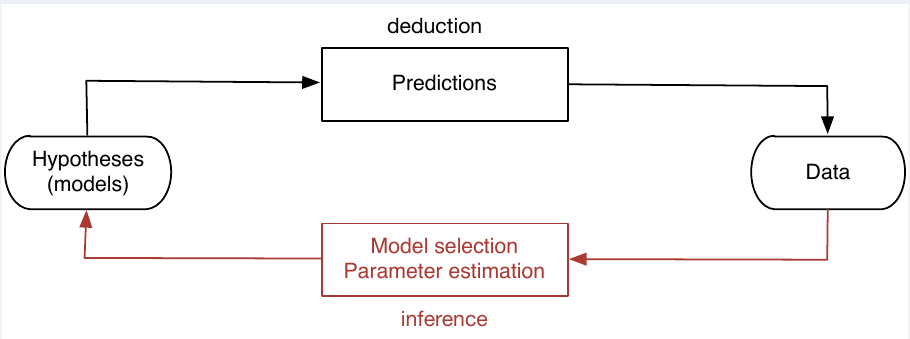
\includegraphics[scale=0.5]{immagini/schema-modello.png}
	\caption{Schema generale della derivazione di un modello di ML}
\end{figure}\\
l'algoritmo di predizione viene chiamato in ML \textbf{modello}. Il processo è tipicamente iterativo: a partire dai dati si fa un ipotesi su come è fatto il modello, si misurano le prestazioni ed eventualmente si migliora il modello in qualche modo.\\\\
\section{Supervised learning}
Quello di cui stiamo parlando è il supervised learning: il training set è un insieme di vettori con un valore target associato ad ogni elemento, sarà una matrice X, con dimensione nxd, per ognuno degli elementi ci sarà il vettore target di n elementi.\\Geometricamente è come se avessi un insieme di n punti in uno spazio di d dimensioni ed a cui è associato un valore, voglio quindi trovare un modo per dividere lo spazio di d dimensioni: sempre nel caso sesso vs altezza, peso, gli elementi saranno punti in uno spazio 2D, alcuni maschi e femmine. Vorrei avere un metodo, ovvero una decomposizione dello spazio in regioni in cui ad ogni regione associo un valore del target così che quanto arriva un nuovo elemento, in base alla regione dove cade so il valore del target.\\Partiziono quindi lo spazio del dominio D in regioni, è solo un modo diverso di vedere la cosa.\\Abbiamo poi un'ulteriore divisione, in base al fatto che il valore target sia reale o discreto:
\begin{itemize}
	\item nel primo caso si parla di \textbf{regressione}: ho un inseme di caratteristiche su un immobile, a partire dal quale voglio conoscere il valore sul mercato
	\item parlo altrimenti di classificazione, nel caso in cui il numero di classi sia finito, come nel caso della perdizione M/F (classificazione binaria)
\end{itemize}
A questo punto, abbiamo il training set e vogliamo dedurre come poter predirre il target a partire dalle feature, anche qui abbiamo una divisione:
\begin{itemize}
	\item cerchiamo di ottenere una funzione $y()$, che ha come dominio un vettore di feature e restituisce un codominio: y: $\mathbb{R} \rightarrow \mathbb{R}$, arriva un $x$ di cui non conosco il target e faccio $y(x)$
	\item approccio probabilistico in cui cerchiamo di ottenere una distribuzione di probabilità per ognuno degli elementi, a partire dalla sue feature. Tale distribuzione sarà su tutti i valori del target.\\Pensando all'esempio di prima, la persone è alta 1.68 e pesa 57kg, l'algoritmo deve dirmi che col 73\% è femmina e col 100-73 è maschio. Questo caso è molto più informativo del primo, possiamo anche stimare meglio l'affidabilità che è legata in qualche modo alla varianza della distribuzione.\\Inoltre, se il sistema da una distribuzione di probabilità dei possibili valori target, dire Maschio/Femmina serve un metodo che stabilisce effettivamente il valore target da assegnare (serve quindi un passo in più).\\Magari non conviene semplicemente assegnare in base alla probabilità più alta, ad esempio quando gli errori non pesano allo stesso modo: se prendiamo l'esempio del covid, se il sistema è probabilistico ci saranno degli errori che sono falsi positivi o falsi negativi.\\In questo contesto i due errori non pesano allo stesso modo.\\C'è un discorso che ha quindi a che fare con la gestione del rischio, che rende possibile l'attuazione di politiche ulteriori e quindi rende questo approccio più informativo del primo
\end{itemize}
\section{Unsupervised learning}
Qui non abbiamo il valore del terget, quindi il problema non è prevedere il valore del target ma: ho un insieme di valori di elementi e in qualche modo voglio riuscire ad estrarre dell'informazione che viene rappresentata da quell'insieme di elementi.\\Supponiamo di avere elementi in uno spazio 2D, dall'osservazione del dataset possiamo stabilire due cose (metti magari disegno):
\begin{itemize}
	\item il fatto che gli elementi possono raggrupparsi in gruppi abbastanza separati fra loro. Possiamo osservare la tendenza a raggrupparsi in così detti \textbf{cluster} un analisi che cerca di capire se avviene tale raggruppamento è il \textbf{clustering}.\\Un esempio è cercare ad esempio di raggruppare in un certo numero di cluster, vedere in quanti cluster sta uno stesso elemento, l'idea è dire che gli elementi si raggruppano in qualche modo per via di una certa variabile che non vediamo e determina tale raggruppamento.
	\item possiamo osservare che gli elementi non sono completamente sparsi su tutto il dominio, ma sono introno ad una retta, gli elementi più o meno sono intorno lì.\\Quindi i valori delle feature stanno più o meno intorno ad uno spazio di dimensione 1.\\C'è quindi una regolarità in quanto le i valori delle feature non sono totalmente indipendenti fra loro, la variabile è quindi una sola e che determina la posizione del punto sulla retta. L'idea è che le feature con cui rappresentiamo gli elementi non sono fra loro indipendenti, quindi in realtà i gradi di libertà veri sono di meno rispetto al numero di feature considerate.\\Potremo avere una situazione in cui i punti non sono proprio sulla retta ma intorno ad essa, il che vuol dire che le feature dipendono anche da altro e non da una sola variabile.\\Questo si chiama \textbf{feature selection} o \textbf{feature extraction}.\\Caso limite: dei punti che hanno tutti la stessa valore della y e diversi della x, andiamo quindi ad estrarre un sotto insieme dalle feature ottenendo dei vettori di dimensione $d'< d$.
	\item selezione di outlayers: un outlayer è un valore molto distante da tutti gli altri, ad esempio quando si fa analisi di log cerchiamo di trovare outlayers. \textsf{\textbf{un nero in Cina e misuri il suo bel cazzone e quello degli altri (l'ha scritto Gian Marco)}}. Definiamo una distribuzione di probabilità sui dati, per poi verificare la probabilità di ciascun elemento, se tale probabilità è bassa vuol dire che il punto è "strano" 
\end{itemize}
\section{Reinforcement learning}
Apprendimento in cui ciò che vogliamo apprendere non è: consideriamo il caso supervisionato come raffronto, nel cui caso vogliamo predirre il valore del target.\\In questo caso vogliamo tirare fuori un algoritmo, una serie di passi che possono essere eseguiti: un esempio tipico è l'apprendimento automatico del movimento del drone, quindi a guida autonoma. Non è possibile elencare cosa fare in corrispondenza ad ogni singolo evento, ma si porta il sistema in cui ogni cosa avviene, in corrispondenza in cui ogni cosa che accade l'algoritmo deve prendere una decisione per poi massimizzare (una funzione?? Bho, non lo approfondiremo).\\Ha a che fare con tutti i sistemi che operano nel tempo.\\C'è una funzione di premio o penality per ogni possibile stato: il sistema quando parte prova a vedere dove va a finire ed apprende che una certa sequenza di mosse porta ad una situazione vantaggiosa o svantaggiosa

\section{Approfondimento nel supervised learning}
\subsection{Loss function}
Siamo nel caso supervisionato: abbiamo quindi un insieme di possibili valori, il dominio $\mathscr{X}$ che è l'insieme degli oggetti che vorremmo poter etichettare. Ogni oggetto è modellato con un vettore di feature, intendiamo:
\begin{itemize}
	\item dimensione è la grandezza del vettore di feature.
	\item il numero di fetaure è la dimensionalità
\end{itemize}
L'insieme delle label è $\mathscr{Y}$, il training set è una matrice $\mathscr{X}$ in cui le righe corrispondono ai vettori di feature ed il target è un vettore colonna.\\Tutto ciò che diremo parte da un modello generale della situazione: abbiamo un insieme di dati che è il tranining set, che sarà quindi un campione (in termini statistici), quindi assumiamo che tali oggetti rappresentino un campione sul dominio dei possibili valori.\\Avremo quindi il training set 
$\mathscr{T}$ = \{(\textbf{x$_1$}, t$_1$),...,(\textbf{x$_n$}, t$_n$)\}.\\Denoteremo poi con \textbf{X} la matrice delle feature:\\
\textbf{X} = $\begin{pmatrix}
	- & \textbf{x$_1$} & -\\
	 & . & \\
	 & . & \\
	 & . & \\
	 - & \textbf{x$_n$} & -\\
\end{pmatrix}$\\\\mentre il vettore delle labels \textbf{t} = $\begin{pmatrix}
\textbf{t$_1$}\\
.\\
.\\
.\\
\textbf{t$_n$}
\end{pmatrix}$\\
\\\\L'estrazione sarà avvenuta usando una qualche distribuzione di probabilità che non conosciamo, che è la distribuzione degli elementi ed è come aver preso a caso gli elementi secondo tale distribuzione, quindi la probabilità di prendere l'elemento è proprio secondo quella della distribuzione.\\Quindi $\forall x, p_{\mathscr{D}_1}(x)$ è la probabilità di estrarre x data la distribuzione $\mathscr{D}$ (ovvero la probabilità che il prossimo elemento campionato nel training set sia proprio \textbf{x}).\\Per la label: supponiamo di aver estratto x secondo $\mathscr{D}_1$, allora il target relativo verrà estratto da un urna dove ci sono tutti i valori target, con una distribuzione di probabilità $\mathscr{D}_2$ che sarà però condizionata ad X, quindi $p_{\mathscr{D}_2}(t|\boldsymbol{x})$, questo per ciascuna $t \in \mathscr{Y}$.\\Assumiamo quindi di avere $\mathscr{D}_1$, $\mathscr{D}_2$ che è condizionata, di aver preso le feature x da $\mathscr{D}_1$ e per ognuno di essi di aver estratto la label da $D_2$: $p_{\mathscr{D}_2}(t|x)$, quindi per il momento supponiamo che ci sia una funzione incognita $f$ tale che $t_i = f(\boldsymbol{x_i})$.\\Supponiamo di avere $x \in \mathscr{X}$, questo $x$ ha una sula label corretta che chiamiamo $y$.\\Supponiamo di fissare un predittore, ovvero (in questo caso) una funzione $h$ che preso x fornisce una previsione. Possiamo fare $h(x)$ e confrontare il valore predetto con quello corretto e stabilire l'errore che sto facendo (ovvero un \textbf{NUMERELLO}). Possiamo fare questo confronto nel training set, per stabilire quanto sto sbagliando usiamo una funzione predefinita: 
\begin{equation}
	L: \mathscr{Y} \text{x} \mathscr{Y} \rightarrow \mathbb{R}
\end{equation}
che chiamiamo \textbf{funzione costo}.\\Avremo poi che il rischio della predizione è 
\begin{equation}
	\mathscr{R}(\hat{y}, y) = L((h\text{x}), y)
\end{equation}\\
Più sarà elevato il valore dato dalla funzione loss e più stiamo sbagliando, consideriamo tutto come funzione di $h$: fissato il punto, cambiando h otteniamo una previsione diversa e quindi un valore diverso di loss per cui voglio scegliere la h tale per cui il valore di errore sia il più piccolo possibile.\\Il punto rimane fisso, vario $h$ e scelgo quella con loss migliore e questa è l'ottimizzazione.\\Il \textbf{rischio della predizione} è il valore della funzione loss, ovvero il rischio che ci si assume nel fare la predizione $h(x)$ invece di y.\\Il problema è trovare, di tutte le funzioni di predizione quella "buona" e non basta considerare solo un punto, occorre sceglierne una che tenda a comportarsi bene per tutti i punti, ovvero una per cui \textbf{la media del rischio} è più bassa possibile, in modo che se estraggo punti a caso e la media è la più bassa, la funzione può essere quella buona:
\begin{equation}
	R(\hat{y}, \boldsymbol{x}) = E_ {\mathscr{D}_2}[L(\hat{y}, y)] = \int\limits_{\mathscr{Y}} L(\hat{y}, y) \cdot p_{\mathscr{D}_2}(y|\boldsymbol{x}) dy
\end{equation}
oppure nel caso discreto\\
\begin{equation}
	R(\hat{y}, \boldsymbol{x}) = E_ {\mathscr{D}_2}[L(\hat{y}, y)] = \sum\limits_{\mathscr{Y}} L(\hat{y}, y) \cdot p_{\mathscr{D}_2}(y|\boldsymbol{x})
\end{equation}\\
dove $L(\hat{y}, y)$ è il costo nel caso in cui il valore target è quello e la previsione è quella che fa la $h(y)$ (sarebbe il valore di loss).\\La predizione ottima, in questo caso, è quella per cui il rischio è il più basso possibile: arriva $x$, supponiamo che la label sia M/F. Una politica è dire che, se rispondo M ed è M abbiamo un certo valore della loss, ma abbiamo anche una certa probabilità associata che magari è bassa. Nel caso F, abbiamo del rischio ma associato alla probabilità più alta. Consideriamo quindi la somma delle due cose, rispondendo sempre la cosa che fa minimizzare il rischio e quindi 
\begin{equation}
	y^*(\boldsymbol{x}) = \underset{\hat{y}}{argmin} \mathscr{R}(\hat{y}, \boldsymbol{x}) =  \underset{\hat{y}}{argmin} E_{\mathscr{D}_2}[L(\hat{y}, y)] 
\end{equation}
quanto io sbaglio dipende dal rischio e dal valore reale, non conosciamo il valore reale ma sappiamo di quanto sbagliamo in base alla probabilità di avere label M/F per la x:
\begin{equation}
	y^*(\boldsymbol{x}) = \underset{\hat{y}}{argmin}L(\hat{y}, f(\boldsymbol{x}))
\end{equation}
o nel caso generalizzato
\begin{equation}
	y^*(\boldsymbol{x}) = \underset{\hat{y}}{argmin} E_{\mathscr{D}_2}[L(\hat{y}, y)] = \underset{\hat{y}}{argmin} \int\limits_{\mathscr{Y}} L(\hat{y},y) \cdot p_{\mathscr{D}_2}(y | \boldsymbol{x})dy
\end{equation} nel caso generale.\\\\
Questo si chiama \textbf{stima Bayesiana}, ma chiaramente il tutto non è applicabile perché non si conoscono $\mathscr{D}_2$ e $p(y|\boldsymbol{x})$.\\Quindi, possiamo allargare il discorso dicendo che rispetto all'insieme dei possibili elementi definiamo il rischio medio, che sarà
\begin{equation}
	\mathscr{R}(h) = E_{\mathscr{D}_1,f}[L(h(\boldsymbol{x}), y)] = \int\limits_{\mathscr{X}} L(h(\boldsymbol{x}), f(\boldsymbol{x})) \cdot p_{\mathscr{D}_1}(\boldsymbol{x}) d\boldsymbol{x}
\end{equation}
o nel caso generale:
\begin{equation}
	\mathscr{R}(h) = E_{\mathscr{D}_1,\mathscr{D}_2}[L(h(\boldsymbol{x}), y)] = \int\limits_{\mathscr{X}}\int\limits_{\mathscr{Y}} L(h(\boldsymbol{x}), y) \cdot p_{\mathscr{D}_1}(\boldsymbol{x}) \cdot p_{\mathscr{D}_2}(y | \boldsymbol{x}) d\boldsymbol{x}dy
\end{equation}
ovvero mediamo il rischio sui possibili valori e troviamo un valore che è il rischio atteso che possiamo avere nel momento in cui usiamo quel predittore su un valore estratto a caso.\\Questo è quanto ci aspettiamo di sbagliare: la funzione loss ci dice quanto sbagliamo se usiamo il predittore h nel momento in cui arriva l'elemento x.\\Otteniamo quindi un rischio che deriva semplicemente da h (funzione di funzione).\\Ho un insieme di possibili funzioni h, prendiamo quella che minimizza questo rischio perché minimizza quanto ci aspettiamo di sbagliare se l'elemento è preso a caso ed il target associato è preso a caso.\\L'$h$ è quindi quella che minimizza $\mathscr{R}(h)$ nel mondo concettuale.\\Il punto è che $\mathscr{D}_1$, $\mathscr{D}_2$ (o $f$) non sono note, ma abbiamo un campione estratto da quell'insieme e quindi non possiamo calcolare il rischio dalle distribuzione etc... ma calcolare la media aritmetica della funzione loss rispetto ad ogni elemento del training set. Facciamo quindi l'approssimazione nel finito
\begin{equation}
	\mathscr{R}_\mathscr{T}(h) = \frac{1}{|\mathscr{T}|} \sum\limits_{(x,y) \in \mathscr{T}} L(h(x),t)
\end{equation}
ottenendo quindi il costo di usare quella funzione di predizione $h$ usando $x$, per poi passare a tutti gli altri $x$.\\È tutto funzione di $h$.\\Arriviamo quindi a dire che il predittore che scegliamo viene preso mediante operazione di ottimizzazione, quindi è quello che minimizza il rischio calcolato sul training set, quindi dipende dal traning ma anche dalla funzione loss. Quindi va fissato come calcolo l'errore (la funzione loss), il training set (quindi c'è la variabilità).\\Ma cerchiamo $h$ dove? In che dominio?Questo ha a che fare col passo successivo ovvero $h^*$ che è la $h$ che minimizza il rischio empirico su un insieme $\mathscr{H}$ di possibili funzioni.\\$\mathscr{H}$ vuol dire "in che insieme di predittori cerco":
\begin{equation}
	h^* = \underset{h \in \mathscr{H}}{argmin}\mathscr{R}_{\mathscr{T}}(h)
\end{equation}
Abbiamo quindi due assunti importanti:
\begin{itemize}
	\item lo spazio dei predittori in cui cerchiamo
	\item la funzione che rappresenta l'errore
\end{itemize}
vogliamo scegliere il predittore, ovvero la funzione $h$ che fa si che la $\overline{\mathscr{R}_{\mathscr{T}(h)}}$ minima.\\Il problema di apprendimento è quindi un problema di minimizzazione: cerchiamo nell'insieme $\mathscr{H}$ la funzione che minimizza l'errore.\\Ma questo matematicamente è un po' scomodo, quindi vedremo che in realtà si fa altro.\\La scelta del dominio dei predittori fra cui cerchiamo il migliore è una aspetto importante, ci possiamo chiedere 
	\begin{itemize}
		\item qual è l'aspetto sull'apprendimento della dimensione di $\mathscr{H}$
		\item come definire lo spazio delle funzioni in modo che sia "abbastanza semplice" calcolare il minimo
	\end{itemize}

\subsection{Scelta dell'insieme delle funzioni} 
Ci sono una serie di considerazioni di carattere teorico, evidentemente la classe delle ipotesi $\mathscr{H}$ verrà presa per qualche motivo relativo probabilmente a qualche conoscenza pregressa che dice quale $\mathscr{H}$ usare, ma in realtà potremmo anche andare per tentativi: cerchiamo la migliore funzione in un certo contesto, magari poi cambiamo $\mathscr{H}$ e cerchiamo in un altro contesto e così via... per poi confrontare.\\Nei casi più diffusi, dopo avere definito $\mathscr{H}$  individuare la $h^*$ è qualcosa che avviene in maniera algoritmica (librerie che lo fanno da un punto di vista sperimentale), ma se vogliamo applicare metodi di ML avverrà che cambieremo $\mathscr{H}$, dove questo può voler dire cambiare proprio la definizione delle funzioni, la loro struttura, oppure degli aspetti parametrici delle funzioni: ad esempio, per una regressione, potremmo considerare tutte le funzioni da $\mathbb{R} \rightarrow \mathbb{R}$, quindi potrei:
\begin{itemize}
	\item considerare solo polinomi di grado 1
	\item solo polinomi di grado 2, quindi funzioni della stessa classe, ma che variano per un parametro che caratterizzano la classe stessa
	\item usare funzioni trigonometriche, cambiando totalmente la struttura quindi
\end{itemize}
Scegliendo una certa $\mathscr{H}$ ci si aspetta che lì ci sia un predittore che si comporta bene, allora la cosa migliore che si possa fare sembrerebbe essere definirla più ricca possibile, al limite prendere tutte le funzioni $f: \mathscr{X} \rightarrow \mathscr{Y}$.\\Supponiamo di avere quindi grande libertà nello scegliere la funzione predittore, supponiamo di voler fare una classificazione binaria, dato un training set $\mathscr{T}$ = (\textbf{X}, t) la funzione di costo più naturale é $L(y,t)$ = 0 se $y=t$ ed 1 altrimenti (aggiusta), quindi naturalmente conto quante volte sbaglio.\\Il rischio è quindi il numero atteso di errori di classificazione, il rischio empirico è la media del numero di elementi di $\mathscr{T}$ che sono classificati male.\\Assumiamo poi che nella popolazione, la metà degli elementi siano M e la metà F, quindi 
\begin{equation}
	p(t=1 | \boldsymbol{x}) = \frac{1}{2}
\end{equation} 
per \textbf{x} $\in$ $\mathscr{X}$, quindi l'ipotesi è che le due classi siano bilanciate.\\Vogliamo trovare un buon classificatore binario, data una funzione di costo che sia il numero di errori.\\Facciamo un classificatore che si comporta così:
\begin{itemize}
	\item guarda tutti gli elementi di $\mathscr{T}$
	\item a tutti gli elementi che hanno target 1 assegna valore 1
	\item assegna 0 altrimenti 
\end{itemize} 
formalmente quindi, il valore di loss sarà definito come:\\
$
L(y,t) =
\begin{cases}
	0 & \text{se } y = t\\
	1 & \text{altrimenti}
\end{cases}
$
\\\\Il rischio empirico del predittore è 0, perché non sbaglia mai sul training set, ma è proprio sul rischio empirico che noi ci basiamo.\\Da un punto di vista della popolazione, se supponiamo che il $\mathscr{T}$ sia piccolo, grosso modo l'errore è $\approx \frac{1}{2}$, sbaglia tutti i maschi che non sono nel $\mathscr{T}$.\\Quindi non va bene, il problema è che il predittore è troppo specifico per il training set, è stato costruito per rispondere bene sul training set.\\Potremmo quindi dire di rispondere sempre a caso, ma anche qui va male perché è sempre $\frac{1}{2}$, non sto tenendo conto del training set.\\Quindi non posso non tenere conto del training set ma nemmeno tenerne conto troppo. La seconda cosa è perché manca la \textbf{generalizzazione}: il resto del mondo non è uguale a ciò che già so, magari assomiglia ma fino ad un certo punto.\\Quindi nel ML occorre tenere conto dei dati ma non tenerne troppo conto. Il fenomeno per cui il prediottore si comporta troppo meglio su $\mathscr{H}$ che sui dai è l'\textbf{overfitting}: il predittore predice molto bene cosa sa e molto male ciò che non sa.\\Mentre il caso opposto, ovvero si tiene poco conto dei dati, presumibilmente il predittore predirrà male tutto ed è l'\textbf{underfitting}.\\La funzione così definita non va bene perché la libertà su $h$ è eccessiva, quindi "ci suggerisce" che se lo spazio delle ipotesi è molto vasto, troppo vasto allora si troverà una funzione che predice perfettamente il training set ma magari in questo modo è troppo specializzata e non riesce a predirre il resto.\\Ma se lo spazio delle ipotesi è troppo piccolo, magari la migliore funzione che trio fuori predice male.\\esempio: voglio fare regressione, supponiamo che gli elementi siano questi:\\
\begin{figure}
	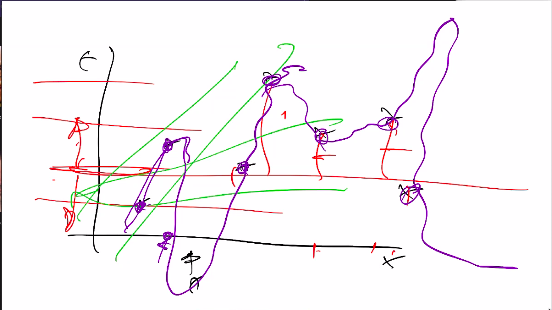
\includegraphics[scale=0.5]{immagini/under_over_fitt.png}
	\caption{Esempio di unerfitting (rette e funzioni costanti) ed overfitting (polinomio viola di grado n)}
\end{figure}\\\\
se l'errore fosse la somma delle distanze, allora questa cambierà ma saremmo lì. È quindi una classe ristretta di funzioni, ovvero tutte le costanti. Posso passare a tutte le rette, la migliore retta sarà meglio della migliore costante (regressione lineare).\\Ancora meglio, le curve quadratiche: le distanze diminuiscono, perché ho più gradi di libertà.\\I 7 punti, preso un polinomio di grado 6 li copro tutti e quindi il miglior polinomio di grado 6 è unico e passerà per tutti i punti ma avrà un andamento strano, dovrà molto "aggiustarsi" ma allora per un punto che non fa parte del training set è molto sballata.\\Con le rette siamo in underfitting, con i polinomi di "grado pari a" siamo in overfitting.\\\\Possiamo avere quindi le seguenti considerazioni:
\begin{itemize}
	\item $\mathscr{H}$ troppo grande porta all'overfitting, si parla di complessità dell'insieme ed ha a che fare tipicamente con il numero di parametri
	\item $\mathscr{H}$ è piccolo abbiamo underfitting
\end{itemize}
Collegato a questo concetto c'è il \textbf{trade-off} fra bias e varianza: se devo effettuare apprendimento, definisco un insieme di funzioni e poi estraggo un training set a caso dalla popolazione e guardando ad esso cerco di trovare la migliore funzione.Cosa può accadere:
\begin{itemize}
	\item caso banale, ho una sola funzione. Risponde sempre 0, il predittore migliore della classe (che è lui perché è da solo) predice sempre allo stesso modo e quindi questo è indipendente dal training set per quella classe.\\È un caso estremo, ma al variare del training set la migliore funzione può cambiare, nel caso delle rette orizzontali ne possiamo ottenere una diversa ma la qualità della predizione non sarà molto diversa.\\Quindi più p meno tutti i possibili predittori sbagliano un po' tutti allo stesso modo, il predittore può anche variabile un po' ma lo sbaglio commesso sarà sempre molto simile e parlo quindi di bias.
	\item il caso opposto è quello in cui ho un polinomio di grado elevato, quindi il predittore scelto è fortemente dipendente dal training set.\\In caso di oevrfitting l'algoritmo di machine learning fornisce un predittore che cambia molto al variare del training set e parlo quindi di varianza.\\Ho sempre un insieme di predittore talmente ampio in cui il predittore, per ogni nuovo training set lo predice molto bene ma cambia sempre la variare del training set.
\end{itemize}
Ho sempre queste due componenti in gioco: il bias, che è l'errore sistematico ovvero quanto qualunque predittore che posso trovare sbaglia e la varianza, ovvero quanta differenza di prestazioni c'è fra due predittori derivati però da due training set diversi.\\\\Prendiamo come esempio la figura:\\
\begin{figure}
	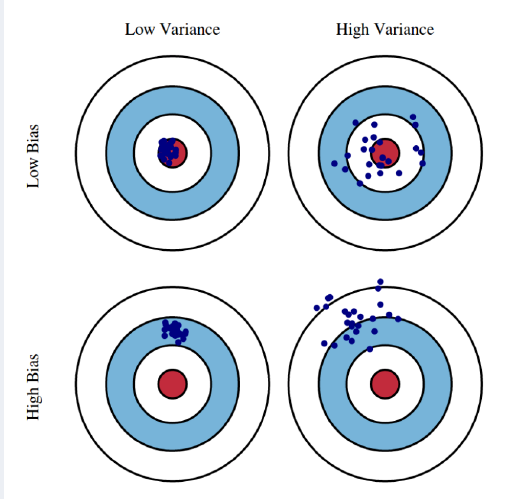
\includegraphics[scale=0.7]{immagini/bias_var.png}
	\caption{Possibili composizioni di bias e varianza}
\end{figure}\\\\
nel caso 2, il bias è basso perché nel complesso la "freccetta" lanciata prende nel centro.\\Il caso 3, nel ML, vuol dire che c'è poca dipendenza dal training set da cui si apprende ma tutti i predittori tendono a sbagliare in modo significativo (caso della retta orizzontale).\\Quindi il rischio associato può essere diviso in 
\begin{equation}
	\mathscr{R}(h^*) = \epsilon_B + \epsilon_V 
\end{equation}
relative a bias e varianza, dove:
\begin{itemize}
	\item $\epsilon_B$ è il rischio minimo ottenibile da ogni $h \in \mathscr{H}$, è determinato solo dal bias indotto ed è indipendente dal training set
	\item $\epsilon_V$ è la differenza fra il rischio minimo in $\mathscr{H}$ ed il rischio associato al miglior prediottre di $\mathscr{H}$ relativamente al training set.\\È una misura di quanto un predittore calcolato per un particolare training set approssima il miglio predittore possibile.
\end{itemize}
Una rappresentazione grafica è la seguente:\\
\begin{figure}
	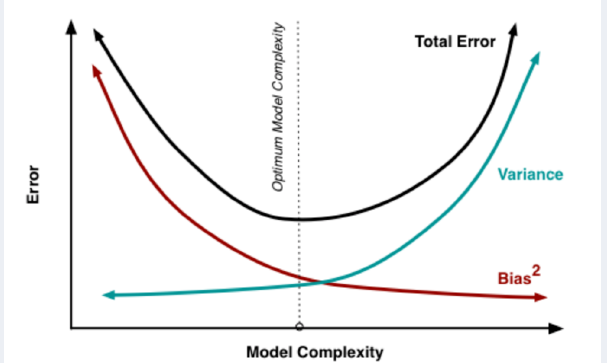
\includegraphics[scale=0.7]{immagini/err_complex.png}
	\caption{Complessità del modello ed errore}
\end{figure}\\\\
È possibile vedere che se siamo in underfitting siamo in bassa varianza ed elevato bias, quindi abbiamo modello molto semplici (sinistra del grafico), quindi il bias (curva rossa) è alto e la varianza è bassa.\\L'errore totale è alto.\\Aumentando la dimensione di $\mathscr{H}$ e quindi la complessità del modello, abbiamo il contrario ovvero bias basso ma variabilità elevata.Le due composte insieme danno sempre errore elevato.\\Esiste una zona intermedia in cui i due fenomeni si bilanciano, quindi bias e varianza non troppo elevato
\subsection{Calcolare la h*}
Altra questione importante è come calcolare la $h^*$.\\Se lo spazio è di funzioni, occorre ottimizzare su di esso e non ci piace, quindi cerchiamo di riportati ad un'ottimizzazione su uno spazio di punti definendo $\mathscr{H}$ in modo parametrico: la struttura è data, ad esempio tutti i polinomi di un certo grado, differiscono perché cambiano i parametri.\\Lo spazio di funzioni è quindi in realtà uno spazio di punti, ad esempio ogni retta è un punto nello spazio (w$_0$, w$_1$).\\Diventa quindi un problema di ottimizzazione standard, matematicamente abbiamo che se lo spazio di funzioni è definito sulla base di k parametri, allora ogni funzione è un punto in uno spazio a k dimensioni.\\Dato un training set e data una funzione loss, ognuno di quei punti ha un valore di un rischio empirico: la situazione è quella per cui ho un insieme di punti in uno spazio a k dimensioni per cui ho assegnato ad ognuno dei punti il valore del rischio empirico, vado quindi da $\mathbb{R}^k \rightarrow \mathbb{R}$.\\Dobbiamo quindi fare:
\begin{equation}
	\theta* = \underset{\theta \in \Theta}{argmin} \overline{\mathscr{R}_{\mathscr{T}}}(h_{\theta})
\end{equation}
le o sono delle teta.\\Abbiamo ancora l problema di dover minimizzare una funzione di k variabili: per farlo, si va a derivare, ma abbiamo dei problemi:
\begin{itemize}
	\item le derivate non servono a calcolare il minimo, ma i punti in cui la derivata è nulla e che può essere un punto di flesso, un punto di max o di min
	\item inoltre, non danno il minimo assoluto
\end{itemize}
possiamo quindi fare la derivata parziale ed annullarla, magari useremo funzioni che per come sono fatte sappiamo che lì dove è nulla la derivata troviamo un minimo.\\A k variabili annulliamo le k derivate parziali, abbiamo quindi un sistema kxk.\\Il sistema si risolve se lineare e questo dipende dalla funzione di partenza, ma l'approccio basato sull'analisi non si applica nella maggior parte dei casi (\textbf{e per fortuna aggiungerei}), allora si può andare con i metodi numerici che è quello che tipicamente si applica in ML: si cerca di trovare un minimo locale nella funzione mediante un metodo iterativo.
\subsubsection{Metodo di discesa del gradiente}
Supponiamo di fare una passeggiata in montagna, in ogni punto c'è un'altitudine associata. Vogliamo arrivare in cima, ma guardando solo intorno a noi, per salire cerchiamo di vedere dove la pendenza è più alta a salire.Ad ogni passo siamo ad una diversa quota ed iterativamente, da un punto di vista matematico abbiamo un punto, a cui è associato un valore della funzione, vogliamo massimizzare e quindi si vede nell'intorno di quel punto dove è la direzione in cui la funzione aumenta di più.\\Ce lo dice il gradiente, ovvero l'insieme delle derivate parziali rispetto a tutte le componenti tramite algoritmo individua la direzioni più alta.\\Iterativamente:
\begin{itemize}
	\item parto da un punto
	\item valuto il gradiente in quel punto, è un vettore di k dimensioni che punta in qualche direzione
	\item il nuovo punto è dato dal precedente + il gradiente nuovo
\end{itemize}
Nel caso del minimo, abbiamo un "-"
\begin{equation}
	\theta^{(k+1)} = \theta^{(k)} - \eta \nabla_{\theta} J(\theta) \bigg\rvert_{\theta = \theta^{(k)}}
\end{equation}
dove $\theta = \theta^{(k)}$ e la $\eta$ è un parametro di tuning che identifica il passo con cui si avanza.\\Scomposto pe ogni parametro:
\begin{equation}
	\theta^{(k+1)} = \theta^{(k)} - \eta \dfrac{\partial J(\theta)}{\partial \theta_i}\bigg\rvert_{\theta = \theta^{(k)}}
\end{equation}
per ogni $\theta_i$.\\Visivamente:\\
\begin{figure}
	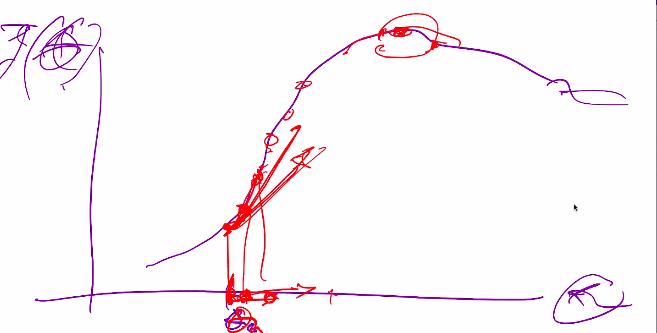
\includegraphics[scale=0.6]{immagini/disc_gradiente.png}
	\caption{Rappresentazione grafica del metodo}
\end{figure}\\\\
\\partiamo da $\theta^{(0)}$, $\theta^{(1)}$ sarà dato da $\theta^{(0)}$ + il valore della derivata. Se la derivata è elevata, quindi se c'è pendenza si farà un passo più lungo, altrimenti si avanzerà a passi più corti.\\Arrivati ad un punto di massimo la derivata è 0, il punto successivo è uguale al precedente e ci si ferma, ma non funziona esattamente così perché si va per passi ma approssimativamente si va così.\\La funzione da ottimizzare è il rischio empirico, che è la somma delle funzioni loss.\\Abbiamo poi il caso della minimizzazione del rischio empirico:
\begin{equation}
	\theta_i^{(k+1)} = \theta_i^{(k)} - \eta \frac{\partial}{\partial\theta_i} \frac{1}{|\mathscr{T}|} \sum\limits_{(x,t)\in \mathscr{T}} L(h_{\theta}(x), t)\bigg\rvert_{\theta = \theta^{(k)}} =  
	\theta_i^{(k)} - \frac{\eta}{|\mathscr{T}|} \sum\limits_{(x,t)\in \mathscr{T}} \frac{\partial}{\partial\theta_i} L(h_{\theta}(x), t)\bigg\rvert_{\theta = \theta^{(k)}}
\end{equation}
\\il rischio empirico è definito come la somma del costo per ogni punto del training set, ogni volta che facciamo un passo nella discesa del gradiente va valutato questo valore che vuol dire andare a considerare tutti gli insiemi del training set. Ad ogni passo ho una nuova funzione di predizione, si confronta con la funzione loss e si ripete, è quello che si chiama \textbf{batch gradient descent}: 
\begin{equation}
	\theta_i^{(k+1)} = \theta_i^{(k)} - \frac{\eta}{|B_r|} \sum\limits_{(x,t)\in \mathscr{T}} \frac{\partial}{\partial\theta_i} L(h_{\theta}(x), t)\bigg\rvert_{\theta = \theta^{(k)}}
\end{equation}
guardare ad ogni passo ogni elemento del training set non scala bene per training set molto grandi.\\La soluzione è non considerare cosa succede sempre per tutti i punti ma solo su un sotto-insieme, non sarà uguale ma è gestibile.\\Si divide in pezzi il training set ed ogni volta entra in gioco il rischio empirico calcolato solo su una parte del training set.\\Partiamo ad esempio dai primi mille punti, facendo la media su quei primi mille. Aggiorniamo, abbiamo una nuova funzione e ripetiamo ma sui secondo mille, guardando sempre ad un mini-batch e che viene fatto nelle reti neurali.\\Quello che può accadere è che ci siano delle oscillazioni intorno allo 0, in quanto operativamente derivata pari a 0 non si ha e più è corto il passo e più ci si avvicina, per cui converrebbe un $\eta$ più piccolo,ma se è piccolo ci mettiamo di più e quindi c'è un tradeoff.\\In base al metodo, possiamo perfezionare la lunghezza del passo.
\subsection{Approcci probabilistici}
In molti casi vogliamo un metodo che ci dia una distribuzione per ogni valore del target, ovvero per ogni valore avere delle probabilità.\\Quindi non vogliamo una $h(x)$ ma una $p(t|x)$, questi sono approcci che danno più informazione ed a cui possiamo poi attaccare delle regole di decisione a posteriori.\\L'idea è più o meno la stessa, quindi consideriamo una classe di possibili distribuzioni condizionali e cerchiamo di capire qual è la migliore secondo una misura.\\A questo punto, trovato $p^*$ dato un nuovo elemento \textbf{x} calcoliamo $p^*(y | \boldsymbol{x})$. Come per le funzioni, dobbiamo definire una classe delle possibili distribuzioni condizionate ed i problemi sono gli stessi di prima:
\begin{itemize}
	\item come definire la classe
	\item come definire la misura della qualità della distribuzione.
\end{itemize}
potrei però pensare di effettuare la mia predizione magari mettendo insieme le predizioni di più predittori, ad esempio quelle di tutti quelli possibili.\\Serve quindi un modo poi per comporre le risposte per trovarne una singola: è l'approccio che da un lato viene chiamato \textbf{ensamble}, notare che nel fare questo per fare le cose per bene occorrerebbe pesare la predizione fatta da ogni predittore sulla base dell'affidabilità fatta da ognuno di essi.\\C'è quindi un aspetto di composizione delle predizioni fatte da ognuno dei singoli modelli ognuna pesata dalla qualità predittiva sempre pesata in base al training set.\\Questo approccio segue la stessa idea, anche se sviluppata in maniera diversa, ovvero dell'apprendimento Bayesiano ma con una formulazione matematica più elegante.\\Se lo vediamo sulle distribuzioni di probabilità, ci sarà un qualche tipo di misura della qualità di quella distribuzione rispetto al training set (come per il rischio empirico): se supponiamo d avere questa valutazione di qualità $q(p, \mathscr{T})$, allora potremmo dire, per effettuare la valutazione, considerare tutte le distribuzioni di probabilità pesate per questa valutazione della qualità.\\Se anche la $q$ ha la forma di una distribuzione di probabilità allora otteniamo un prodotto delle probabilità: $q(p) \cdot p(y|x)$ posso ottenere il valore atteso di questo prodotto integrando (che è l'approccio Bayesiano).
\subsection{Analisi notebook}
Abbiamo diverse misure che ci permette di determinare la qualità della predizione:
\begin{itemize}
	\item Accuratezza: $\frac{\text{\# items classified correctly}}{\text{\# items}}$. Problema: supponiamo che il 99\% delle cifre nel training set siano tutti 9.Facendo un classificatore su questo training set dirà sempre 9, che su questo training set avrà Accuracy 0.99, quindi se la situazione è di classi sbilanciate e consideriamo l'Accuracy, questo tende a distorcere il comportamento del classificatore che tenderà a classificare di più in quel modo. Dobbiamo bilanciare il fenomeno dello sbilanciamento, ma anche fatto questo non possiamo considerare l'Accuracy come una buona metrica.
	\item Precision class $i$: $\dfrac{\text{\# items from class i classified correctly}}{\text{\# items classified as class i}}$
	
	\item Recall class $i$: $\dfrac{\text{\# items from class i classified correctly}}{\text{\# items from class i}}$: abbiamo un trade off: possiamo avere recall 1 della classe 0 predicendo tutti gli elementi come appartenenti alla classe 0 ma la Precision sarà bassissima.
	
	\item F-score class $i$: $\dfrac{\text{Precision classe i} \times \text{Recall classe i}}{\text{Precision classe i}+\text{Recall classe i}}$. Mette insieme Precision e Recall, utilizzando la media armonica: $\frac{a\cdot b}{a + b}$ (se consideriamo a e b)
\end{itemize}
Il caso in cui il modello che otteniamo ha valori per le metriche relative a training set e testing set simili  vuol dire che non siamo né in underfitting né in overfitting.
\subsection{Loss function e training set}
La funzione di loss è tale per cui data una coppia di valori del codominio (uno corretto e l'altro predetto) ci restituisce un valore reale, che misura il costo che noi associamo al fatto di usare y al posto del valore corretto t.\\Nel supervised learning, ci fornisce una misura delle qualità di predizione effettuata dalla funzione $h$, quindi il rischio che associamo alla coppia x,y non è che il valore della loss function.\\Il rischio empirico è (vedi sopra) questo è quello che prendiamo come misura della qualità predittiva della funzione h.\\A questo punto nella fase di apprendimento il rischio empirico è minimizzato rispetto alle predizioni che effettua la funzione h, consideriamo la h parametrizzata, quindi la funzione loss complessiva è la somma delle loss applicate ai vari elementi: (copia), per ogni elemento ho una diversa loss function, vista come funzione di $\theta$. Come facciamo a minimizzare: ci piacerebbe trovare un minimo globale, usando l'analisi matematica e trovare il valore che ponga tutte le derivate a 0 (con la garanzia che i punti siano di minimo, quindi guardando la derivata '' oppure l'hessiano ma \textbf{GRAZIE A DIO NON SI RIESCE AD APPLICARE}). In linea di principio facciamo la derivata parziale rispetto ad uno dei coefficienti ed azzeriamo. Ci sono almeno due problemi:
\begin{itemize}
	\item possiamo avere diverse soluzioni per il sistema di equazioni
	\item possono essere difficili o impossibili da calcolare analiticamente
\end{itemize}
quindi possiamo introdurre metodi numerici iterativi mediante la \textbf{discesa del gradiente}: mi muovo nello spazio dei coefficienti $\Theta$ ed applico un aggiornamento che deriva dalla valutazione del gradiente nel punto precedente, guardo alla derivata parziale del rischio empirico nel punto e modifico il valore attuale.\\L'approccio rende in linea di principio possibile trovare il minimo globale, abbiamo però problemi di:
\begin{itemize}
	\item[1] punti di sella e punti di flesso
	\item[2] quanto rapidamente di converge
\end{itemize}
possiamo dire che, alla fine, questo dipende dalla funzione di loss e quindi scelta tale per cui che l'unico punto a derivata nulla sia unico ed un minimo ho risolto il punto 1, non avrò nemmeno minimi locali che non sono globali.\\Se non possiamo scegliere questa funzione, allora si vede che in molti casi se abbiamo anche una sella il metodo ne viene fuori, o anche se si prende un minimo locale tipicamente quel minimo locale non è lontano da quello globale, usando dei modelli con un certo livello di complicazione.
\subsection{Funzione di loss}
La funzione di loss prende origine dal concetto di convessità: qualunque coppia di punti di un insieme, tutti quelli che stanno sulla retta appartengono all'insieme. (copia immagine, insieme non convesso ha ad esempio un "buco" sulla destra). Diciamo che una funzione è convessa se l'insieme dei punti che sono sopra è convesso. Questo vuol dire che presi due punti sulla funzione e collegandoli, tutti i punti sono al di sopra della funzione. (copia immagine e definizione, è quella che diremmo a derivata '' positiva).\\Assumendo che la funzione $f(x)$ sia convessa, si può mostrare che c'è un solo minimo globale (ad esempio nella parabola). Se è strettamente convessa, ovvero i punti spora sono la funzione sono sempre strettamente maggiori, allora esiste solo un minimo locale che è globale e risolvere (copia) ci da questo minimo.\\Vogliamo questo tipo di funzioni loss, ovvero che siano strettamente convesse, se sono convesse la situazione è più debole perché ci possono essere più minimi locali che però sono tutti globali in quanto hanno lo stesso valore (?).\\Caso semplice ma rilevante è se la $f(x)$ è una funzione quadratica.\\In molti modelli semplici usiamo una funzione loss quadratica, ma ora dire questo vuol dire che $L(\theta, x_i, y_i)$ è quadratica ed il rischio empirico è la somma di queste funzioni. Esiste un teorema che dice che la somma di funzioni convesse è una funzione convessa.\\Quindi stiamo dicendo che usando questo tipo di funzioni, il rischio empirico sarà a sua volta convessa e quindi avrà un solo minimo locale che è globale e quindi applicando il metodo della discesa del gradiente, quando si arriva sul minimo locale si arriva anche sul globale.\\Ora quindi si possono scegliere le funzioni di loss con vari criteri
\subsubsection{Alcune funzioni di loss comuni}
Il primo caso è quello delle regressioni: una funzione loss tipicamente usata è il quadrato dell'errore (copia) che è un modo per stimare la distanza. Il quadrato ci dice che possiamo non tenere conto del segno.\\Abbiamo quindi il seguente rischio empirico (copia).\\Se facciamo in particolare regressione lineare, allora $h(x)$ è combinazione lineare dei valori delle feature (copia), dove w è il vettore dei coefficienti ed otteniamo la funzione di costo (che voglio minimizzare) quindi (copia).\\Vogliamo trovare fra tutti i valori dei coefficienti w e b quelli per cui l'espressione è minima. N.B: l'espressione ha come variabili w e b, mentre x e t sono dati.\\Per trovare il minimo possiamo cercare di calcolare il gradiente, (copia)\\\\Un'altra funzione loss è la differenza in modulo (copia), sempre convessa.\\Serve che la funzione gradiente sia definita per ogni punto, altrimenti non saprei come muovermi per avanzare (derivata definita in ogni punto ?).\\\\Abbiamo poi la Huber loss, che dentro è quadratica e poi fuori diventa lineare. La funzione quadratica tende a penalizzare molto più di questa funzione una differenza significativa, quindi se si sbaglia il costo assegnato all'errore cresce molto di più rispetto alla funzione valore assoluto, quindi la scelta è quanto penalizzare gli errori se diventano grandi.
\subsubsection{Funzioni di loss per la classificazione}
In questo caso, possiamo avere diversi casi (predizioni di valore, distribuzione etc...) assumiamo di considerare classificazione binaria, che dirà quale dei due valori è corretto per le due classi ed il valore predetto è la probabilità assegnata di appartenenza ad una delle classi.\\Una prima funzione di loss è la così detta loss-01, ovvero (copia): il valore predetto è t e quello corretto è y, assumiamo che y sia 1 o -1 e vediamo il segno del valore predetto: se positivo, allora è 1 e se il valore corretto è 1 allora non abbiamo errori.\\Prendiamo quindi il valore corretto e ne facciamo il segno, per poi vedere il valore della funzione segno. Se t = .3, allora sng(t) è 1, se quindi la classe vera è 1 (y=1) allora non ho errori (0), altrimenti ho un errore (1). Sto quindi contando gli errori, la rappresentazione è la seguente: (copia).\\La funzione ha dei problemi:
\begin{itemize}
	\item non è convessa
	\item non ha la derivata definita in qualunque punto (non è nemmeno continua in ogni punto)
\end{itemize}
non possiamo quindi adottare la tecnica della discesa del gradiente, perché se becchiamo gradiente 0 \textbf{non ce muoviamo più dar punto. È come cercare la cima der monte in pianura}.\\Se assumiamo una funzione di predizione lineare otteniamo una loss: (copia), allora trovare il valore di w che minimizzi l'errore è NP-hard. Quindi la funzione non va bene, allora possiamo usare delle funzioni che assomigliano alla 01, che sono funzioni \textbf{surrogate}: queste funzioni approssimano la loss-01 "da sopra", quindi per ogni coppia predizione, target assegna un valore superiore di quello della loss-01, approssima quindi sempre da sopra.\\È convessa, è derivabile in ogni punto cambia fra le diverse surrogate la forma ed il peso che viene dato agli errori.\\\\La prima che possiamo considerare, non surrogata, è la perceptron loss: nella loss-01 diamo 0 in caso di successo ed 1 come errore, quindi diciamo che se non "ci prende" il valore è proporzionale a quanto il classificatore abbia sbagliato la predizione.\\Se la classe è 1 ed il valore predetto è -5, il valore del costo è altro, se è -15 è ancora più alto.\\La loss è fatta così (copiala)\\questa funzione di costo non è però surrogata perché il suo costo non maggiora quello della 01 in determinati intervalli, è continua, il gradiente è continuo quasi ovunque, è convessa ma non ci piace tantissimo.\\\\La spostiamo di 1 con la Hinge loss: è surrogata, è anch'essa continua e col gradiente continuo quasi dovunque ed è convessa.\\Questa è una funzione di loss spesso usata (copia tutto), viene molto usata in modelli di classificazione importanti, ma ha però un problema ovvero in un punto la derivata non è definita.\\\\Abbiamo poi la Sqaure loss (copia): una funzione di questo tipo è che se la classe è 1 quanto più t è negativo e quanto più l'errore è grande. Ma se il valore predetto sta dalla parte giusta, quanto più sta dalla parte giusta tanto più aumenta l'errore.\\\\Log loss: (copia) molto usata, è il tipo che ci piace perché maggiora la 01, è continua, a derivata continua. Questa funzione tende a penalizzare sempre di più quanto più si sbaglia ma dalla parte della predizione corretta penalizza sempre di meno tanto più quanto il valore corretto è nella direzione corretta.\\\\Infine, l'exponential loss: altro tipo di funzione tipo la Log, l'andamento è simile e c'ha le stesse caratteristiche, quindi componendo con la somma la derivata sarà sempre definita e sempre convessa. La differenza con la Log è che la log penalizza meno gli errori grandi rispetto alla Exponential.\\\\\\Qui le vediamo tutte insieme (copia)\\cambiando funzione loss che utilizzo, cambierà il risultato.




























\end{document}